\chapter{Context and Objectives}
\section{Javascript}

\subsection{Explosion of Javascript popularity}

\subsubsection{In the beginning}

Javascript was created by Brendan Eich in 10 days in May 1995, while he was working at Netscape.
The inital name of the project was Mocha, and then switched to LiveScript when released to the public in September 1995.
The name Javascript was later adopter to leverage the trend around Java.
Indeed, Java was considered the new hot web programming language at this time.
% TODO read Javascript the good parts

Microsoft released a concurrent implementation of Javascript in June 1996 in their browser Internet Explorer 3.
They changed the name to JScript, to avoid trademark conflict with Oracle Corporation, who owns the name Javascript.
But the differences between the two implementations made difficult for a script to be compatible for both.
Netscape submitted Javascript to Ecma International for standardization in November 1996.
In June 1997, Ecma International released ECMA-262, the first specification of EcmaScript, the standard for Javascript.
% TODO more on the Ecma specification please

It was designed as a simple language to attract unexperienced developers.
By opposition to Java or C++, which target professional developers.
% TODO reformulate that

\subsubsection{Rising of the unpopular language}

Javascript started as a programming language to animate web pages.
It was used as a script language to implement short interactions.
The main usage was for validate form on the client, avoiding unnecessary calls to the server.

In 2005 James Jesse Garrett released Ajax: A New Approach to Web Applications, a white paper coining the term Ajax. \cite{Garrett2005}
Ajax, consists in using Javascript to dynamically request and refresh the content of a web page.
This paper point the trend in using this technique, and explain the consequences on user experience.
Indeed, an application able to react to the user without completely refreshing the page, is bringing the web closer to a native application.
At the time, some important web application started using this technique.
The most important being Gmail, the google mail client.

At roughly the same time famous Javascript libraries were released with the goal to fill the differences between browsers implementations of Javascript.

% TODO there is probably a lot more to write about this transition :
% - Google used a lot of Ajax in its sites (gmail, google maps, orkut and so on ...)
% - jquery / prototype ... all the famous library that helped Javascript gain in popularity
% - ... ?

\subsubsection{Current situation : complete world domination}

All modern web browsers now include a Javascript interpreter, making Javascript the most ubiquitous runtime in history. \cite{Flanagan2006}

But the fact that Javascript is the language of the web, also made it famous in the open source communities.
Javascript is the language counting the most repository on github, and is the most tagged language in StackOverflow.

Languages like Java and C/C++ are in active use in the software industry.
Javascript on the other hand, is rising from the open source community and is slowly taking over the software industry as well.

With the release of HTML5, the importance of Javascript was completely acknowledged.
It marked the consideration of the web as viable alternative for desktop clients.
And with the mobile trends, most products are now released as a mobile apps, and a web application.

The web is now the norm.
It is the application platform.
And because Javascript is programming language of the web, it is \textit{de facto} the language of choice to develop technologies.\ftnt{http://blog.codinghorror.com/javascript-the-lingua-franca-of-the-web/}

Some might consider HTML5 is not yet ready to build complete application on mobile, where condition in terms of performance, and accessibility are not as good as on the desktop.
But even in these cases, Javascript seems to remain the language of choice, as proven with React Native\ftnt{https://facebook.github.io/react-native/}, from Facebook, who prone the "learn once, write anywhere", in opposition to the "develop once deploy everywhere of the web".


\paragraph{Isomorphic Javascript}

https://www.meteor.com/

https://facebook.github.io/flux/

\paragraph{Reactive}

http://facebook.github.io/react/

Code reuse.
Why it never worked ?





https://www.destroyallsoftware.com/talks/the-birth-and-death-of-javascript

The Atom editor is written in Javascript node.js.



Now, major PaaS (which one) support node.js by default.

Heroku support Python, Java, Ruby, Node.js, PHP, Clojure and Scala

Amazon Lambda Web service support node.js in priority.


>>> News :

npm raises 8m.
http://techcrunch.com/2015/04/14/popular-javascript-package-manager-npm-raises-8m-launches-private-modules/

% >>> I want to say that Javascript is now broadly used.
% Let's just look at the numbers : Javascript is the most popular language on Github, and npm has more package than any other package manager.
% Javascript has the more broadly deployed runtime.
% ... and so on
% >>> the conclusion is : Javascript is now a major language, and it is more than worth the consideration we are giving it in this PhD thesis.



\subsection{Overview of the language}

Javascript was released in a hurry, without a strong and directive philosophy.
During its evolution, it snowballed with different features to accommodate the community, and the usage it was made on the web. As a result Javascript contains various, and sometimes conflicting, programming paradigms.
It borrow its syntax from a procedural language, like C, and the object notation from an object-oriented language, like Java, but it provides a different inheritance mechanism, based on prototypes. Most of the implementation adopt an event-based paradigm, like the DOM\ftnt{http://www.w3.org/DOM/} and node.js\ftnt{https://nodejs.org/}.
And finally, event though it is not purely functional like Haskel, Javascript borrows some concepts from functional programming.

In this section, we focus on the last two programming paradigm, functional programming and event-based programming.
Javascript exposes two features from functional programming.
Namely, it treats functions as first-class citizen, and allows them to close on their defining context, to become closures.
We will explain these two features in details, and see how they are highly attractive to program in an event-based paradigm.

\subsubsection{Functions as First-Class citizens}

\cit{All problems in computer science can be solved by another level of indirection}{Butler Lampson}

Javascript treats function as first-class citizens.
One can manipulate functions like any other type (number, string ...).
She can store functions in variables or object properties, pass functions as arguments to other functions, and write functions that return functions.

The most common usage examples of these features, are the methods \texttt{Map}, \texttt{Reduce} and \texttt{filter}.
In the example below, the method \texttt{map} expect a function to apply on all the element of an array to modify its content, and output a modified array.
A function expecting a function as a parameter is considered to be a higher-order function. \texttt{Map}, \texttt{Reduce} and \texttt{Filter} are higher-order functions.

\begin{code}
  [4, 8, 15, 16, 23, 42].map(function firstClassFunction(element) {
    return element + 1;
  });
  // -> [5, 9, 16, 16, 24, 43]
\end{code}

Higher-order functions provide a new level of indirection, allowing abstractions over functions.
To understand this new level of abstraction, let's briefly summarize the different abstractions on the execution flow offered by programming paradigms.
In imperative programming, the control structures allow to modify the control flow. That is, for example, to execute different instructions depending on the state of the program.
Procedural programming introduces procedures, or functions. That is the possibility to group instructions together to form functions.
They can be applied in different contexts, thus allowing a new abstraction over the execution flow.
% It encourages to abstract program states so that the same function can be applied in different places to apply its behavior.

So, higher-order functions add another level of abstraction.
It allows to dynamically modify the control of the execution flow.
The ability to manipulate functions like any other value allows to abstract over functions, and behavior.
% TODO continue this, there is a lot to say about HOF

Higher-order functions replace the needs for some Object oriented programming design patterns.\ftnt{http://stackoverflow.com/a/5797892/933670} Though object oriented programming doesn't exclude higher-order functions.

They are particularly interesting when the behavior of the program implies to react to inputs provided during the runtime, as we will see later.
Web servers, or graphical user interfaces, for examples, interact with external events of various types.

% TODO transition : higher-order functions makes use of closure to implement the lexical scope in mutable programming languages. (reformulate)

\subsubsection{Closure}

\cit{An object is data with functions. A closure is a function with data.}{John D. Cook}

Closures are indissociable from the concept of lexical environment.
To understand the former, it is important to understand the latter first.

\paragraph{Lexical environment}

A variable is the very first level of indirection provided by programming languages and mathematics.
It is is a binding between a name and a value.
Mutable like in imperative programming to represent the reality of memory cells, or immutable like in mathematics and functional programming.
These bindings are created and modified during the execution.
They form a context in which the execution takes place.
To compartmentalize the execution, a context is also compartmentalized.
A certain context can be accessed only by a precise portion of code.
Most languages defines the scope of this context using code blocks as boundaries.
That is known as lexical scoping, or static scoping.
The variables declared inside a block represent the lexical environment of this block.
These lexical environments are organized following the textual hierarchy of code blocks.
The context available from a certain block of code, that is set of accessible variable, is formed as a cascade of the current lexical environment and all the parent lexical environment, up to the global lexical environment.

% TODO draw the schema for a lexical environment here

\paragraph{Javascript lexical environment}
\ftnt{http://www.ecma-international.org/ecma-262/5.1/\#sec-10.2}

Javascript implement lexical scoping with function definitions as boundaries, instead of code blocks.
The code below show a simple example of lexical scoping in Javascript.

\begin{code}
  var a = 4;
  var c = 6;
  function f() {
    var b = 5;
    var c = 0;
    // a and b are accessible here.
    return a + b + c;
  }

  f(); // -> 9

  // b is not accessible here :
  a + b + c; // -> ReferenceError: b is not defined
\end{code}

Lexical scoping, or statical scoping, implies that the lexical environment are known statically, at compile time for example.
But Javascript is a dynamic language, it doesn't truly provide lexical scoping.
In Javascript, the lexical environments can be dynamically modified using two statements : \texttt{with} and \texttt{eval}.
We explain in details the Javascript lexical scope in section \ref{??? Compiler stuff}

\paragraph{Closure}

A closure is the association of a first-class function with its context.
When a function is passed as an argument to an higher-order function, she closes over its context to become a closure.
When a closure is called, it still has access to the context in which it was defined.
The code below show a simple example of a closure in Javascript.
The function \texttt{g} is defined inside the scope of \texttt{f}, so it has access to the variable \texttt{b}.
When \texttt{f} return \texttt{g} to be assigned in \texttt{h}, it becomes a closure.
The variable \texttt{h} holds a closure referencing the function \texttt{g}, as well as its context, containing the variable \texttt{b}.
The closure \texttt{h} has access to the variable \texttt{b} even outside the scope of the function \texttt{f}.

\begin{code}
  function f() {
    var b = 4;
    return function g(a) {
      return a + b;
    }
  }

  var h = f();
  // b is not accessible here :
  b; // -> ReferenceError: b is not defined

  // h is the function g with a closure over b :
  h(5) // -> 9
\end{code}


% TODO continue with closure


% TODO transition, Higher-order functions and closures are very handy in turn-based programming


\subsection{Turn-based programming}

Javascript, like most programming languages, is synchronous and non-concurrent. The specification doesn't provide mechanism to write concurrent execution of Javascript.
There is no reference to \texttt{setTimeout} nor \texttt{setInterval}.
These two well-known instructions to asynchronously post-pone execution are provided by the DOM.
Indeed, like for many languages, concurrency is supported and provided by the execution engine.
For example the JVM in the case of Java, or the operating system in the case of C/C++.
These last two languages were mostly used to design CPU intensive applications.
The concurrency model for such application is driven by the need for computing power.
The best concurrency model is the threading model.
It allows to run multiple executions simultaneously to leverage the potential of parallel architectures, and execute faster.
Execution engine provide thread libraries to allow concurrency, like pthreads\ftnt{https://computing.llnl.gov/tutorials/pthreads/} for POSIX operating systems, and the \texttt{Thread}\ftnt{https://docs.oracle.com/javase/7/docs/api/java/lang/Thread.html} class for Java.
But, as we will see in a next chapter, threads are known to be very difficult to manipulate.
It is lucky that Javascript was not seen early as a language to build CPU intensive applications, so it can adopt a different concurrency model.

Indeed, Javascript was used from the beginning to build graphical user interfaces.
Since user interfaces evolved from a simple and sequential user prompt to a full interactive graphical space, the user interacts in a non-sequential way.
The interface needs to display and react to multiple streams of interaction.
% TODO find a good example here

The concurrency need is completely different than for CPU intensive applications, and so is the concurrency model.
Graphical user interfaces often use an event-loop.

When an event-loop is used as the concurrency model, it creates what Douglas Crockford called turn-based programming\ftnt{https://youtu.be/dkZFtimgAcM?t=1852}.

As event-loop was never used in CPU intensive applications, there was no need to extend to the multi-thread.
An event-loop is single-threaded, therefore, it always has exclusive access to its memory.
The concurrency is in a time-sliced fashion, each turn has an exclusive access on the memory by design.
And it is never preempted.
The event-loop let each event execute until it yield execution.
The event-loop provide concurrency without the need for synchronization on the form of mutual exclusions, and locks.
% TODO reformulate this paragraph, it is currently badly written.

However, it has a cost.
Each turn needs to be executed fast, so as to avoid the event-queue to congest on events waiting for their turn.


% TODO GUIs hardly ever congest the event-loop, because if the programmer is not so bad, event are fast, and there is usually not so much event : the graphical space is often limited to the attention of a single user.
% However, in the case of web application, there is a lot much more events to process.
% So much in fact, that the congestion of a single event-queue (see USL) is often impacting the latency, and the reactivity of the application.
% At this point, it is interesting to split into multiple event-queue.
% Continue integrating the scalability / concurrency, and follow to the problematic.


Now the browser has a thread-like concurrency model as well, on the form of web workers\ftnt{http://www.w3.org/TR/workers/}.


As said above, most implementations of Javascript feature an event-based programming paradigm.
The DOM\ftnt{http://www.w3.org/DOM/} and node.js\ftnt{https://nodejs.org/} are the most famous examples.


HOF allows Continuation Passing Style, which is particularly useful in a turn-based programming language such as node.js javascript.
% TODO continue to say a lot about CPS



\subsubsection{the Javascript event-loop}

Web pages are graphical environment offering multiple area of interaction for the user.
Because of this multiplicity, the traditional linear programing model doesn't hold anymore.
Graphical systems switched from this linear programming model to a different programming model focused on events.

Javascript uses higher-order functions.
It is the ability for a language to manipulate functions like any other value.
This ability is used to register a function to trigger after an event occurred.
An event might be the click on an element of the page, for example.

Such a function is named a callback, a handler, a listener ...
And it shift the programming paradigm from synchronous to asynchronous, which is a big deal.

In synchronous programming, the computation step are executed sequentially, one after the other.
The program execution follows perfectly the program layout written in a linear textual file.

On the other hand, asynchronous programming allows a step back from this linearity.


A multi-threaded system allows the developer to explicitly express the parallelism in the application.
A GOTO statement allows the developer to explicitly express the control flow in the application.


Asynchronous programming allows the program to manage the concurrency of the execution.
Unlike a linear layout of an imperative program, it allows to express more finely the dependencies between instructions.

% James Coglan speak about Promises and the abstraction they allow on the control flow. much interesting, especially at the end.
% https://blog.jcoglan.com/2013/03/30/callbacks-are-imperative-promises-are-functional-nodes-biggest-missed-opportunity/

% >>> I want to say that Javascript is the first language broadly used with this asynchronous paradigm.
% Is asynchronous programming a step before declarative programming ?

\subsubsection{Promises}

% Douglas Crowford on Promises
% https://www.youtube.com/watch?v=dkZFtimgAcM

% The web is polluted with dumb, simple Promises tutorial for Javascript
% It is hard to find the relevant information about how Promises change the programmation paradigm.


\section{Scalability}
  \subsection{Theories}
    \subsubsection{Linear Scalability}
    \subsubsection{Limited Scalability}
    \subsubsection{Negative Scalability}
      \comment{Conclusion : scalability = concurrency + not sharing the resources that grows with the scale}
  \subsection{Concurrency}
    \comment{Concurrency is time slicing or multi-threading)}
    % \subsubsection{Synchronization}
    %   \comment{when there is concurrency inside a same system (so the components are somewhat dependent on each others : causal relation, or state sharing), there is a need for synchronization}
    %   \paragraph{Lock}
    %   \paragraph{Events}
    %   \paragraph{\comment{TODO} others ?}
    \subsubsection{Time-slicing}
      \paragraph{Task management}
      \paragraph{Stack management}
    \subsubsection{Multi-Threading}
      \paragraph{Eventual Consistency}
      \paragraph{Event-based multi-threading}

  \subsection{Scalability outside computer science (only if I have time)}
      \comment{
        If I have time, I would like to try to explain why scalability is at the core of material engagement and information theory,
        and is at the core of our universe : the propagation of Gravity wave is an example : it is impossible to scale
        }

% 
\section{Scalability}
  \subsection{Theories}
    \subsubsection{Linear Scalability}
    \subsubsection{Limited Scalability}
    \subsubsection{Negative Scalability}
      \comment{Conclusion : scalability = concurrency + not sharing the resources that grows with the scale}
  \subsection{Scalability outside computer science (only if I have time)}
      \comment{
        If I have time, I would like to try to explain why scalability is at the core of material engagement and information theory,
        and is at the core of our universe : the propagation of Gravity wave is an example : it is impossible to scale
        }

/EOF

% TODO introduction to this chapter


We define a web service as a computer program whose main interface is based on web protocols, such as HTTP.
Such a service uses resources allocated on a network of computers.
Scalability defines the ability of the service to use a certain quantity of resource to meet a desired performance.
We call system the association of the computer program and the available resources. 
The performance of this system is measured by its latency and throughput.

\subsection{Latency and throughput}

Latency is the time elapsed between the reception of a request, and the sent of the reply.
It includes the time waiting for resources to be free to process the request, and the time to process the request.

Throughput is the number of requests processed by the system by unit of time.

Latency and throughput are linked in a certain way.
If a modification of the web service reduces its mean latency to a half, then the throughput doubles immediately.
It takes half the time to process a request, therefore, the service can process more requests in the same time.
However, if throughput augment, the latency doesn't necessarily decrease.

\subsection{Scalability granularity}

We define a computer program as a set of operations.
In the case of a web service, these operations can be directly requested by the user through the interface.
An operation can cause any other operation to execute.

Because both the resources used and the operations executed are discrete : not infinitely divisible, scalability is inherently discrete.


% TODO scalability granularity ? 
Scalability granularity is the increment of resources.
How the input data can be split up ?
How the program can be deployed on many machines ?






We call system the association of the computer program with the resources


\subsection{Horizontal and vertical scaling}

There is two ways to augment the resources of the system.
Enhance the nodes in the computer network - vertical scaling.
Or add more nodes to the computer network - horizontal scaling.


% TODO how to apply these theory to highly concurrent servers ?
% How does it modify the theories ?

There are three theories, from the most restrictive, to the most general.


% TODO define scalability
Scalability is the property of a computer program to occupy available resources to meet a needed performance.
EIther in Latency, or in throughput.







\subsection{Linear scalability}

Clements et. al. \cite{Clements2013a} prove that a computer program scale linearly if all its operations are commutative.
% Commutative is not parallel. How to go from commutative to parallel ?
Two operations are said to be commutative if they can be executed in any orders, and the same initial state will result in the same final state.
Commutativity implies the two operations to be memory-conflict free, or independent, which is equivalent to say that they can be executed in parallel.

Therefore, to achieve linear scalability, a computer program must be composed of a set of operations that commutes.
Thus, all the operations are parallel, they can be executed simultaneously, on any number of machines as required.

The size of the operations sets the scalability granularity.

However, commutativity is not achievable in real applications.
Even sv6, the operating system resulting from the work on commutative scalability only has 99\% commutativity.
For real application, in the best case, the granularity is coarse, in the worst case, there is no possible commutativity because of shared resources (like a product inventory, or a friend graph).

% TODO continue

\subsection{Limited scalability}

Amdahl introduced in 1967 a law to predict the limitation of speedup a computer program can achieve if a fraction of its code is sequential.
Amdahl worked at increasing the speed of computer clock, while the scientific community was working on improving parallelism of computing machines.

In a set of operations, even if one is non-commutative, it cannot be executed in parallel of any others, the scalability is limited by this operation.

There is a difference if the operation is non-commutative with itself, or only with others.
In the first case, it impose a queuing, while in the second case, it only increase the granularity : you can regroup the non-commutative operation with its subsequents, and form a bigger commutative operation.

% TODO continue

\subsection{Negative scalability}

Gunther generalized Amdahl's law into the Universal Scalability Law.
It includes the parallelization of non-independent operations with the use of synchronization.

It models the negative return on scalability from sharing resources observed in many real world applications.

% TODO continue by explaining the different area of scalability.



\subsection{Eventual Consistency}

To overpass the scalability limits set by the previous rules, it is possible to abandon consistency.
It simply tolerate incoherences between multiple replicas.
The output of an operation can be false while its state is synchronized with the other replicas.

% It is similar to the propagation of sound, light or gravity.
% When an explosion happens, not everybody hears it at the same time : there is inconsistency in the experience.


% TODO continue
% \section{Concurrency}

Javascript, like most programming languages, is synchronous and non-concurrent. The specification doesn't provide any mechanism to write asynchronous nor concurrent execution of Javascript.
There is no reference to \texttt{setTimeout} nor \texttt{setInterval}.
These two well-known instructions to asynchronously post-pone execution are provided by the DOM.
Indeed, like for many languages, concurrency is supported and provided by the execution engine.
For example the JVM in the case of Java, or the operating system in the case of C/C++.
We explore in this section, the different model to provide concurrency.
\comment{when there is the need for concurrency in a system (so the components are somewhat dependent on each others : causal relation, or state sharing), there is a need for synchronization.
If there is no need for synchronization, then there is two independent systems.
So concurrency is first a topology and synchronization (communication?) problem.}
% TODO continue this introduction

\subsection{Two concurrency model}

We distinguish two types of concurrent models, tailored for two types of applications, CPU bound applications, and I/O bound applications.
An example of CPU bound application is a scientific application, like a physics simulation. Such applications rely heavily on the CPU to do calculation on a fixed set of data.
CPU bound applications need concurrency to augment the computing power.
On the other hand, an example of I/O bound application is graphical user interface.
% Since user interfaces evolved from a simple and sequential user prompt to a full interactive graphical space, the user interacts in a non-sequential way.
It needs to display and react to multiple concurrent streams of interaction.
Another example is a web server, it needs to react to multiple concurrent requests.
I/O bound applications need concurrency to keep track of concurrent control flows in multiple contexts.
The difference between the two needs is thin enough for one to be mistaken with the other.
The two well-known models for concurrency are threads and events.
It is know broadly admitted that threads are the better solution for CPU bound applications, while events are the better solution for I/O bound applications.
However, this distinction is not as clearly defined as it seems.
In the next section I explain what characterizes these two models, what are the differences between the two, and how should they be used.

% Particularly, with the massive introduction of parallel architecture, things got a lot more confusing.
% In the next sections I explain the concurrency model for one core, and for multi-core.

% TODO transition

% time-slicing is actually concurrency on a single core, in certain cases, its called en event-loop, in other cases, its called multi-threading.
% Exactly, event-loop is cooperative task management, while threads is preemptive task management
% And multi-threading is actually concurrency on multiple core, in certain cases, its called multi-threading, in other cases, its called message passing.
% Exactly, multi-threading is lock synchronization, while message passing is share nothing.

\subsubsection{Threads and events}

% TODO transition

% This section should present clearly what are threads and event, historically and currently.
% It should be perfectly clear that threads and events are perpendicular to one or multi-core architecture, and that it is also perpendicular to I/O or CPU bound applications.
% both events, and threads can be used on single, or multi-core architecture, for I/O or CPU bound applications.
% The final transition should be about what exactly drive the choice between all this : preemptive task management (for long concurrent computations) versus cooperative task management (for a lot of small concurrent computations).

Threads-based system and event-based system evolved significantly over the last half century.
These evolutions were fueled by the long-running debate about which design is better.
% We try to succinctly and roughly retrace theses evolutions to understand the positions of each community.
% This demonstration show that thread and events are two faces of the same reality.

\paragraph{Thread}

A thread is the smallest representation/embodiment/...? of the execution of a sequence of instructions on a computing core.
It is characterized by a set of registers on this computing core representing the state of the computation.
It is the smallest ... manipulable by a scheduler.




\paragraph{Event}


% TODO 


\paragraph{Thread and Event are not opposed}

% TODO 


Lauer and Needham \cite{Lauer1979} presented an equivalence between Procedure-oriented Systems and a Message-oriented Systems.

Adya \textit{et. al.} analyzed this debate and presented fives categories through which to present the problem \cite{Adya2002}.
These two categories were often associated with thread-based systems and event-based systems.
% TODO not very clear
Their advantages and drawbacks were mistaken with those of thread and events.
Adya \textit{et. al.} explain in details two of these categories that are most representative, Task management and Stack management.
We paraphrase these explanations.


\subsubsection{Time-slicing}


Time-slicing is the technique used by both threads and event based system when they can dispose only of one computing core to achieve concurrency.

\paragraph{Task management}

Consider a task as an encapsulation of part of the logic of a complete application.
All the task access the same shared state.
The Task management is the strategy chosen to arrange the task executions in available space and time.

Preemptive task management executes each task concurrently.
Their executions interleave on a single core, or overlap on multiple cores.
It allows to leverage the parallelism of modern architectures.
This parallelism has a cost however, developers are responsible for the synchronization of the shared memory.
While accessing a memory cell, it must be locked so that no other task can modify it.
Synchronization mechanism impose the developer to be especially aware of race condition, and deadlocks.
These synchronization problems make concurrency hard to program with preemptive task management.

The opposite approach, Serial task management, executes each task to completion before starting the next.
The exclusivity of execution assures an exclusive access on the memory.
Therefore, it removes the need for synchronization mechanism.
However, this approach is ill-fitted for modern applications, where concurrency is needed.

A compromise approach, Cooperative task management, allows tasks to yield voluntarily.
A task may yield to avoid monopolizing the core for too long.
Typically, it yields to avoid waiting on long I/O operations.
It merges the concurrency of the preemptive task management, and the exclusive memory access.
Thus, it relieves the developer from synchronization problems.
But at the cost of dropping parallel execution.

Threads are associated with preemptive task management, and events with Cooperative task management.
For this reason, it is commonly believed that synchronization mechanisms make threads hard to program \cite{Ousterhout1996}.
While it is really Preemptive task management that is responsible for these synchronization problems \cite{Adya2002}.

% TODO define the two
\paragraph{Stack management}

Consider a task is composed of several subtasks interleaved with I/O operations.
Each I/O operation signal its completion with an event.
The task stops at each I/O operation, and must wait the event to continue the execution.
The stack management is the strategy chosen to express the sequentiality of the subtasks.

The automatic stack management is what is mostly used in imperative programming.
The execution seems to wait the end of the operations to continue with the next instruction.
The call stack is kept intact.
This is what is commonly called synchronous programming.

In the manual stack management, developers need to manually register the handlers to continue the execution after the operation.
The execution immediately continues with the next instruction, without waiting the completion of the operation.
It implies to rip the call stack in two functions; one to initiate the operation, and another to retrieve the result.
This is what is commonly called asynchronously programming.


\subsubsection{Multi-Threading}

Multi-threading is the technique used both by threads and events-based system to achieve concurrency when there is multiple computation core.

  \paragraph{Synchronization}

  \paragraph{Eventual Consistency}

  \paragraph{Event-based multi-threading}
  % Transition to the next subsection : 
  % The event-loop makes use of the two concurrency model : multi-threads for I/O and time-slicing for Computation


\subsection{Event-loop}






\subsection{Turn-based programming}
When an event-loop is used as the concurrency model for a partially functional language like Javascript, it creates what Douglas Crockford called turn-based programming\ftnt{https://youtu.be/dkZFtimgAcM?t=1852}.
% TODO then explain why Javascript is a good choice for this ()


\subsubsection{Promises}

% Douglas Crowford on Promises
% https://www.youtube.com/watch?v=dkZFtimgAcM

% The web is polluted with dumb, simple Promises tutorial for Javascript
% It is hard to find the relevant information about how Promises change the programmation paradigm.

\comment{TODO}

\subsubsection{Generators}

\comment{Generators are a way to implement synchronous programming on top of an event-loop (asynchronous programming), like fibers}











A concurrency model well adapted for such applications is the threading model.
It allows to run multiple executions simultaneously to leverage the potential of parallel architectures, and execute faster.
Execution engine provide thread libraries to allow concurrency, like pthreads\ftnt{https://computing.llnl.gov/tutorials/pthreads/} for POSIX operating systems, and the \texttt{Thread}\ftnt{https://docs.oracle.com/javase/7/docs/api/java/lang/Thread.html} class for Java.
But, as we will see in a next chapter, threads are known to be very difficult to manipulate.
It is lucky that Javascript was not seen as a language to build CPU intensive applications, so it remained free of this concurrency model, and can adopt a different concurrency model.
% TODO reformulate this sentence : Javascript was mainly used to build graphical interfaces, and not CPU intensive applications.











% \paragraph{Fibers} -> TODO state of the art








As said above, most implementations of Javascript feature an event-based programming paradigm.
The DOM\ftnt{http://www.w3.org/DOM/} and node.js\ftnt{https://nodejs.org/} are the most famous examples.
% TODO Place this accordingly

Now the browser has a thread-like concurrency model as well, on the form of web workers\ftnt{http://www.w3.org/TR/workers/}.
% TODO place this accordingly, it might be only a footnote

% \subsubsection{Event-loop}

% As event-loop was never used in CPU intensive applications, there was no need to extend to the multi-thread.

An event-loop answer a particular need of concurrency.
It is designed to use a thread of execution, to several 
% TODO spearate well the two notions : thread of execution -> physical, and logical thread of execution -> a suite of instructions to execute.

The event-loop concurrency model is based around a queue of message, named the event-queue, and a thread of execution to process these messages, named the event-loop.
The event-loop process the messages queued on the event-queue one after the other, each during a turn.
A turn consists of the event-loop pulling a message from the event-queue, and executing the callback associated with this message until it yield the execution when finished.
The execution of the callback is never preempted.

An event-loop is single-threaded, callbacks are executed one after the other on the same CPU.
The concurrency is time-sliced.
During the execution of a callback, there is no other simultaneous execution.
Therefor, each callback has an exclusive access to the memory.

Because each callback has exclusive access to the memory, and is never preempted, it can consider the invariant.
% TODO I don't know yet what exactly is an invariant, so please check.
The event-loop provide concurrency without the need for synchronization on the form of mutual exclusions, and locks.
It is often said that the event-loop provide atomic execution / de facto exclusion ... whatever, because of this pattern.

However, there is a limitation to this concurrency model.
Because all callback are executed on the same core, if one takes two much time to complete, the other can't executes, and the program seems to freeze.
Therefore, each turn needs to be executed fast, so as to avoid the event-queue to congest on events waiting for their turn.

GUIs hardly ever congest the event-loop, because if the programmer is not so bad, event are fast, and there is usually not so much event : the graphical space is often limited to the attention of a single user.
However, in the case of web applications, there is a lot much more events to process.
When there is too many concurrent events to process, the event-loop become congested, and the latency of the application increase.
% TODO therefore, it is interesting to split into multiple event-queue.
% TODO only make a point here : start to build the problematic.

% TODO continue about how to program in an event-loop, and why it is so interesting to have HOF.

HOF allows Continuation Passing Style, which is particularly useful in a turn-based programming language such as node.js javascript.
% TODO continue to say a lot about CPS
% CPS leads all the way to Promises \o/






% Web pages are graphical environment offering multiple area of interaction for the user.
% Because of this multiplicity, the traditional linear programing model doesn't hold anymore.
% Graphical systems switched from this linear programming model to a different programming model focused on events.

% Javascript uses higher-order functions.
% It is the ability for a language to manipulate functions like any other value.
% This ability is used to register a function to trigger after an event occurred.
% An event might be the click on an element of the page, for example.

% Such a function is named a callback, a handler, a listener ...
% And it shift the programming paradigm from synchronous to asynchronous, which is a big deal.

% In synchronous programming, the computation step are executed sequentially, one after the other.
% The program execution follows perfectly the program layout written in a linear textual file.

% On the other hand, asynchronous programming allows a step back from this linearity.


% A multi-threaded system allows the developer to explicitly express the parallelism in the application.
% A GOTO statement allows the developer to explicitly express the control flow in the application.


% Asynchronous programming allows the program to manage the concurrency of the execution.
% Unlike a linear layout of an imperative program, it allows to express more finely the dependencies between instructions.

% James Coglan speak about Promises and the abstraction they allow on the control flow. very interesting, especially at the end.
% https://blog.jcoglan.com/2013/03/30/callbacks-are-imperative-promises-are-functional-nodes-biggest-missed-opportunity/

% >>> I want to say that Javascript is the first language broadly used with this asynchronous paradigm.
% Is asynchronous programming a step before declarative programming ?









% http://berb.github.io/diploma-thesis/original/043_threadsevents.html

% On the Duality of Operating System Structures
% http://tolstenko.net/blog/dados/Unicamp/2010.1/mc714/extras/201_recomendada_Lauer-Needham-78-Duality.pdf

% Threads vs. Events
% http://courses.cs.vt.edu/cs5204/fall09-kafura/Presentations/Threads-VS-Events.pdf

% Why Threads Are A Bad Idea (for most purposes)
% http://www.cs.utah.edu/~regehr/research/ouster.pdf

% Why Events Are A Bad Idea (for high-concurrency servers)
% http://static.usenix.org/publications/library/proceedings/hotos03/tech/full_papers/vonbehren/vonbehren_html/

% http://www.usingcsp.com/cspbook.pdf

% Threads Without the Pain
% http://queue.acm.org/detail.cfm?id=1105678


% Cooperative Task Management without Manual Stack Management or, Event-driven Programming is Not the Opposite of Threaded Programming 
% http://static.usenix.org/publications/library/proceedings/usenix02/full_papers/adyahowell/adyahowell_html/

% Retrospective on SEDA
% http://matt-welsh.blogspot.fr/2010/07/retrospective-on-seda.html

% Latency
% http://highscalability.com/latency-everywhere-and-it-costs-you-sales-how-crush-it
% http://blog.gigaspaces.com/amazon-found-every-100ms-of-latency-cost-them-1-in-sales/




% \subsection{About concurrent systems}


% TODO advantage and disadvantages of synchronous and asynchronous programming

What we argue is that synchronous is good because it is linear, it avoids stack ripping.
But asynchronous is good because it allows parallelism by default.


% synchronous programming is good to express linear execution. In parallel that means quite unrelated linear executions.
% asynchronous programming is good to express interleaved parallel execution. It is easy to express small parallel and sequential tasks.


Threads are associated with the automatic stack management, and events with manual stack management.
For this reason, it is commonly believed that threads are easier to program.
\cite{Thread systems allow programmers to express control flow and encapsulate state in a more natural manner} \cite{Behren2003}.
However, the automatic stack management is not exclusive to threads.
Fibers, presented by Adya \textit{et. al.} is an example of cooperative task management with automatic stack management \cite{Adya2002} .
Fibers present the advantage of cooperative task management, without the disadvantage of stack ripping.
That is the ease of programming because of the absence of synchronization, without the difficulty of stack ripping.

We argue that the advantages of manual stack management outweigh its drawbacks for web services.
Because of the numerous I/O operations, parallelism is 


% TODO I split the explenation in thread then events, instead, I should split in task management, then state management




But what is actually highlighted is the automatic state management provided by threads.
And with lighter context change, threads are a good choice which provide parallelism.

Historically, events-based system are associated with manual state management, while threads-based systems are associated with automatic state management.
Manual state management imposed stack ripping \cite{Adya2002}.
With closure, it is not the case anymore.
Events now have automatic state management as well \cite{Krohn2007}.

Now, there is implementation of thread model with cooperative management, with context-switch overhead improved enough to fill the gap with events model.
And there is implementation of event model with automatic state management filling the gap with thread model.
In this condition, we ask, what really is the difference between thread and events.
We argue there is none.
Except the isolation, versus sharing of the memory, which, again is not significant of either.
In the first case, the different execution threads exchange messages, while in the second, they use synchronization mechanism to assure invariants in their states % TODO disambiguation thread is a context for execution, what is a core of execution ?

For a single thread of execution, both model could avoid synchronization through cooperative task management, which assure invariants. % TODO disambiguation
Or avoid procedure slicing (if any) using synchronization.
These are the two ends of a design spectrum.
One end (cooperative task management) fits better for small processing with heavy use of shared resources.
While the other end (synchronization) fits better for long processing with small use of shared resources.
When one end of the design spectrum is used while the other should be used, one might expect unresponsiveness because of too heavy events, or performance fall due to interlocking.

Scalability is achieved through parallelism, which is itself achieved in our case (web servers) through cluster of commodity machines.
% TODO this links exactly to what I wrote on scalability, find a way to merge the two.

With distribution, this design spectrum gets a better contrast. % TODO that is really false, reformulate to get a correct articulation

The synchronization of distributed, shared resources is limited through the CAP theorem  \cite{Gilbert2002a}. % TODO needs to read this.
Partition tolerance is a requirement of a distributed system. %TODO define PA, and find reference http://codahale.com/you-cant-sacrifice-partition-tolerance/#ft2
One needs to choose good latency (availability) or consistency. % Define the CAP theorem, consistency and availability
The CAP theorem is generalized into a broader theroem about\cite{Gilbert2012} % TODO read, and merge within the argumentation (the paper seems really broad, be careful not to dive too deep)

The isolation of resources implies to split the architecture in different stages, like Ninja \cite{Gribble2001}, SEDA \cite{Welsh2000}, or Flash \cite{Pai1999}.
This splitting is difficult for the developer.
The splitting which is good for the machine, is not the same as the one good for the design in modules.

The two ends of this design spectrum presented map directly onto the two kinds of parallelism advocated for scalability.
That is pipeline parallelism, and data parallelism.

Pipeline parallelism is good for data locality, and important throughput. % TODO reference
But each stage adds an overhead in latency. % TODO reference

Data parallelism is good for latency, because one request is processed from beginning to the end without waiting in queues.
But it implies that the different machines share a common database.
Which is a shared resource, and is limited by the CAP theorem.

Both parallelism have advantages and drawbacks, and both could be combined, like in the SEDA architecture. % TODO find the exact reference that says : it is good to use both parallelism to scale
Ultimately, it would be possible to design a design spectrum to choose which kind of parallelism for a set of requirements.
But we leave this for future works.

Splitting an architecture in stages is a difficult process, which prevent future code refactoring, and module modifications.
We argue that the design for the technical architecture, and the design for the human minds should not be the same.
Threads belong to the mental model, the design granularity
Events belong to the execution model, the architecture granularity
  % TODO quote
  It is a mistake to attempt high concurrency without help from the compiler \cite{Behren2003}.
Through compilation, we want to transform an event-loop based program (cooperative task management, no synchronization) into a pipeline parallelism distributed system.
So, basically, we argue that it is possible to distribute one loop event onto multiple execution core.



% TODO Careful, you don't know fibers enough.
% And globally, there is much that you don't know.

% Il y à quelques années, la tendance chez les gros était de se concentrer sur la parallélisation par threads pour gagner en latence.
% Notamment avec Gigaspace.
% Donc en occultant complètement les events, et en utilisant des grosses bases de données comme Dynamo ou Cassandra qui scalent bien.
% Je n'ai pas vraiment trouvé la même tendance pour les events.
% Storm et Spark stream sont à usage plus spécifique.
% Mais ce déséquilibre est peut être simplement dû à l'héritage de l'architecture n-tier.


% MICROSERVICES
% Plus récemment, j'ai trouvé beaucoup de bruit sur les microservices en 2014.
% Ça me paraissait intéressant, en pensant y trouver des arguments pour favoriser les events, et nuancer la tendance précédente.
% Mais j'ai l'impression qu'il s'agit plus d'une question d'organisation humaine que de performance.
% Il me reste à trouver des arguments pour mettre à égalité les deux axes de parallélisation.





% TODO 
% Continue with the hybrid approach : multiple threads for events, and one threads for user code
% See Flash, SEDA, Node.js etc ...






/!\ WARNING
The paper Why events are a bad idea states that :
the control flow patterns used by these applications fell into three simple categories: call/return, parallel calls, and pipelines.
Indeed, it is no coincidence that common event patterns map cleanly onto the call/return mechanism of threads. Robust systems need acknowledgements for error handling, for storage deallocation, and for cleanup; thus, they need a “return” even in the event model.
>> Why is it completly false ?
	 It is crucial to find an answer.
Moreover, Ayda et. al. state that :
For the classes of applications we reference here [file servers and web servers], processing is often partitioned into stages.
Other system designers advocated non-threaded programming models because they observe that for a certain class of high-performance systems [...] substantial performance improvements can be optained by reducing context switching and carefully implementing application-specific cache-conscious task scheduling.


The paper Why events are a bad idea states that :
One could argue that instead of switching to thread systems, we should build tools or languages that address the problems with event systems (i.e., reply matching, live state management, and shared state management). However, such tools would effectively duplicate the syntax and run-time behavior of threads.
>> Well, yes ...
   With the exception of the stack junction.
   The paper on Duality had it right, their graph is correct, but for threads, it cannot be distributed because of stacks, while for events, it can.


Software evolution substantially magnifies the problem of function ripping: when a function evolves from being compute-only to potentially yielding, all functions, along every path from the function whose concurrency semantics have changed to the root of the call graph may potentially have to be ripped in two. (More precisely, all functions up a branch of the call graph will have to be ripped until a function is encountered that already makes its call in continuation-passing form.) We call this phenomenon ``stack ripping'' and see it as the primary drawback to manual stack management. Note that, as with all global evolutions, functions on the call graph may be maintained by different parties, making the change difficult. 
>> Stack ripping is what I am talking about.
   While the stack are joined, it is not possible to distribute.
   If they say that stack ripping is necessary, that means it is not possible to encapsulate asynchronous function into synchronous function.
\section{Seamless Development} \label{chapter3:objectives}
\nt{TODO title not clear enough}


\begin{center}
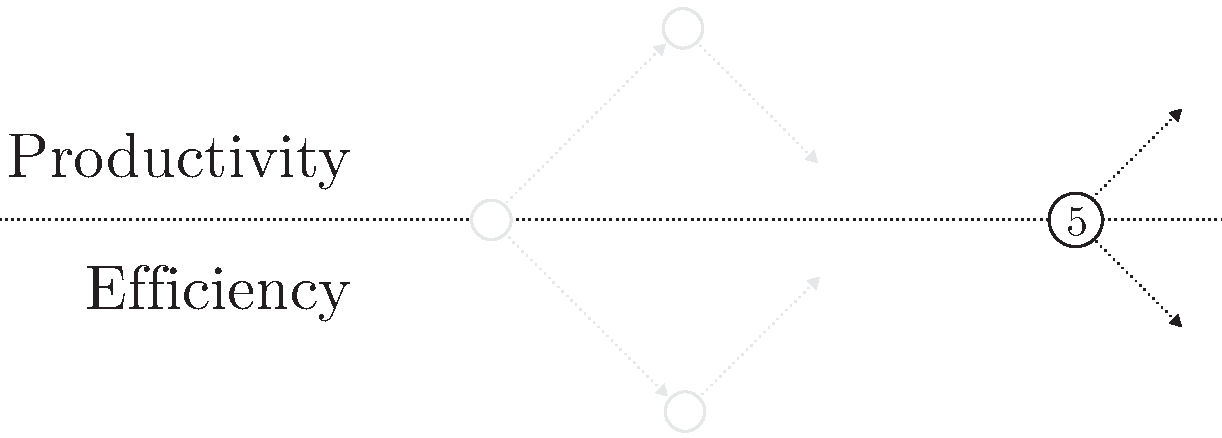
\includegraphics[width=0.6\textwidth]{../ressources/state-of-the-art-5.pdf}
\end{center}

% The objective of this thesis is to find a reconciliation of the two goals, by finding an equivalence between two approaches with different goals, in the case of streaming web applications.

The section \ref{chapter3:software-maintainability} shows that modularity and functional programming, especially higher-order programming and lazy evaluation, are the best organization to improve maintainability of an application.
This organization is best supported by a functional approach.
Indeed, higher-order programming improves readability and maintainability.
However, higher-order programming, and modular programming in general, requires the use of a global memory store.

The section \ref{chapter3:software-performance} shows that to attain scalability, an application needs to be organized to distribute its memory store into independent silos to provide isolation and immutability. Leading to multiply the exclusive accesses.
Still, many works provide this global memory store interface to developers, because it is the best way to support the modularity advocated in section \ref{chapter3:software-design}.
This incompatibility between these two organization, and their goals is responsible for the shifts operated during the life of an application.
Huge developing efforts are made to translate manually from one organization into the other, and to maintain the implementation despites its unmaintainable nature.
% when the most pressing need shift from maintainability to performance, or vice versa.

In section \ref{chapter3:objectives}, we show different tentatives to reconciles the two organizations.
Most are satisfactory for specific domains, such as the high-performance computing.
It is profitable, as the expected speedup of developing an application with an adapted programming model compensates the huge development effort.
%  where it is accepted to spend long time developing an application to use thousands of accelerators to compute heavy calculation, because the expected speedup is profitable, compared to develop an application for all these thousands accelerators.
However, none are satisfactory in the case of web applications because the need for performance is always uncertain.
The development effort is not required at the beginning, hence its cost cannot be justified.
It is only when the audience increases, often with the revenue, that the cost for the development effort can be justified.
This situation illustrate the need for a programming model reconciling the two concerns, of maintainability and performance.
% Indeed, they all are too specific, and require too much from the developer to be accepted at a large scale.

% \comment{Here a table summarizing the different approaches, and the sweet spot.}

Our objectives is to provide seamless development.
3.1 shows that modularity is not scalable but needed.
But compilation can help to get scalable.
3.2 shows that parallelism is not maintainable (no Higher-Order Programming, no lazy evaluation, so no good glue between modules)
But good developers can maintain double representation.
With help from an equivalence or a \textit{compiler} most developers could develop using this double representation, and seamlessly achieving parallelism and maintainability.

\begin{table}
\begin{tabular}{l|l|l|l}
             & Maintainability         & Performance           & Both\\\hline
General      & Functional Programming  & Message-passing       & Loop parallelization\\
Web          & Javascript              & Pipeline architecture & ø
\end{tabular}
\caption{Summary of the state of the art}
\label{tab:chapter3:objectives:summary}
\end{table}

\nt{integrate these paragraphs after the next section}
Our objectives is to find an equivalence between these two organization, specifically for the case of web applications.
To do so, we focus on the Javascript programming language, and specifically, the node.js interpreter.
\nt{TODO not clear}
As explained in the end of chapter \ref{chapter2}, the execution model of Javascript is similar to a pipeline.
We intend to split a node.js application into a parallel pipeline of stages.

The contribution of this thesis is organized in two chapters, as illustrated in figure \ref{fig:chapter3:objectives:roadmap}.
In chapter \ref{chapter4} I present the extraction of a pipeline of operations from a Javascript application.
I show that such pipeline is similar to the one exposed by Promises, and I propose a simpler alternative to the latter called Dues.
However, these operations still require a global memory for coordination so they are not executed in parallel.
In chapter \ref{chapter5}, we present the isolation of the operations into isolated containers called Fluxions. 

\begin{figure}[h!]
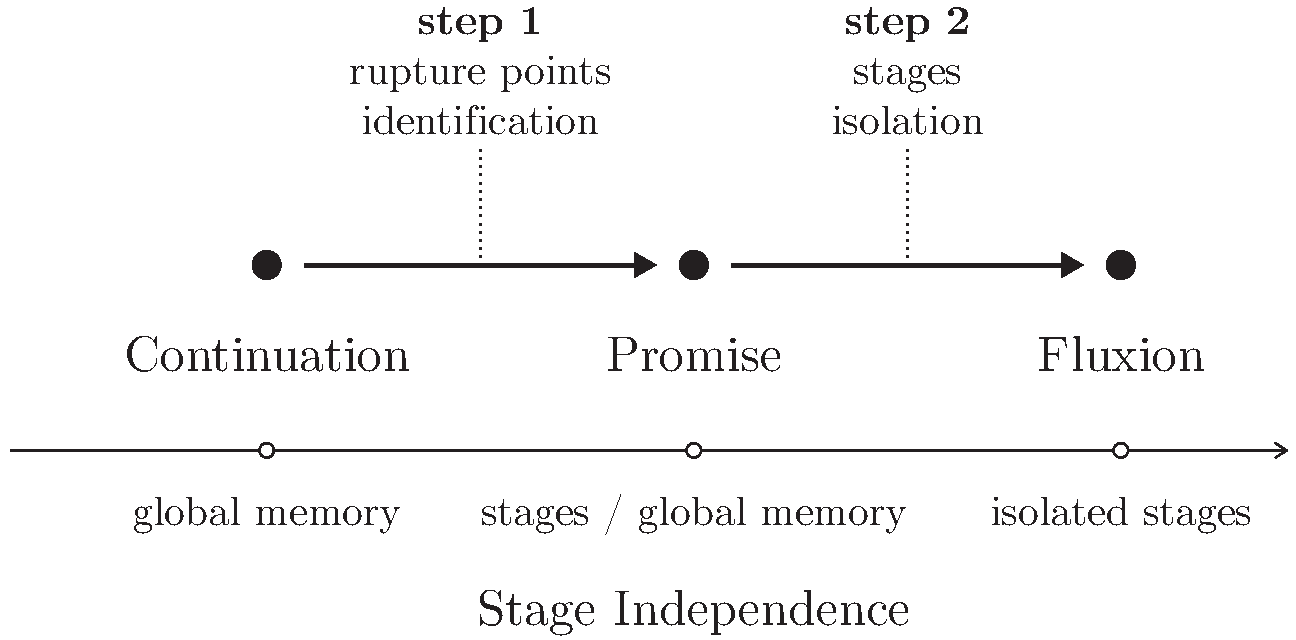
\includegraphics[width=1\textwidth]{../ressources/roadmap.pdf}
\caption{Roadmap for this work}
\label{fig:chapter3:objectives:roadmap}
\end{figure}

\begin{center}
\rule{3cm}{0.4pt}
need integration
\rule{3cm}{0.4pt}
\end{center}

We show that there is no languages that features higher-order functions to improve modularity, a common memory store easy to develop with, but at the same time provides scalable concurrency.

We aim at filling this gap, and for a concrete example, focus our work on the Javascript programing language.
Indeed, Javascript features higher-order functions, is highly-used in concurrent context, but lacks scalable concurrency.








\subsection{Equivalence}

\subsubsection{Rupture Point}

The execution of the pipeline architecture is well delimited in isolated stages.
Each stage has its own thread of execution, and is independent from the others.
On the contrary, the code of the event-loop is linear because of the continuation passing style and the common memory store.
% The message passing linking the callbacks is transparently handled by the event-loop.
However, the execution of the different callbacks are as distinct as the execution of the different stages of a pipeline.
The call stacks of two callbacks are distincts.
Therefore, an asynchronous function call represents the rupture between two call stacks.
It is a rupture point, and is equivalent to a data stream between two stages in the pipeline architecture.

Both the pipeline architecture and the event-loop present these rupture points.
The detection of rupture points allows to map a pipeline architecture onto the implementation following the event-loop model.
To allow the transformation from one to the other, this thesis studies the possibility to detect rupture points, and to distribute the global memory into the parts defined by these rupture points.
The detection of rupture points is addressed in chapter \ref{chapter4}.

\subsubsection{Invariance}

% This transformation is important on two points.
% The conservation of the invariance.
% The equivalence between the coordinations.

The transformation should preserve the invariance as expressed by the developer to assure the correctness of the execution.
The partial ordering of events in a system, by opposition to total ordering, is sufficient to assure this correctness.
% This result was used by Lamport to prove the correctness of distributed systems.
The global memory is a way to assure the total ordering of events, and the message passing coordination is a way to assure partial ordering of events.
Therefore, to assure the correctness of the execution of a system, the state coordination with a global memory is equivalent to message passing coordination.
And it is possible, at least for some rupture points, to transform the global memory coordination into message passing while conserving the correctness of execution.

In order to preserve the invariance assured by the event-loop model after the transformation, each stage of the pipeline needs to have an exclusive access to memory.
The global memory needs not to be split into parts and distributed into each of the stages.
To assure the missing coordinations assured by the shared memory between the stages, the transformation should provide equivalent coordination with message passing.
The isolation and replacement of the global memory is fully address in chapter \ref{chapter5}

% The invariance holds for the whole memory during the execution of each callback.
% As I explained in the previous section, this invariance is required to allow the concurrent execution of the different tasks.
% On the other hand, the invariance is explicit in the pipeline architecture, as all the stages have isolated memories.
% The coordination between these isolated process is made explicit by the developer through message passing.

% I argue that the state coordination between the callbacks requireing a global memory could be replaced by the message passing coordination used manually in the pipeline architecture.
% I argue that not all applications need concurrent access on the state, and therefore, need a shared memory.
% % Specifically, I argue that each state region remains roughly local to a stage during its modification.
% \nt{TODO review that, I don't know how to formulate these paragraphs. Identify the state and the data in the global memory.}

% \subsubsection{Transformation}

% This equivalence should allow the transformation of an event loop into several parallel processes communicating by messages.
% In this thesis, I study the static transformation of a program, but the equivalence should also hold for a dynamic transformation.
% I present the analyzis tools I developed to identify the state and the data from the global memory.
